\section{Introduction}
\label{sec:intro}

Humans effortlessly retrieve keys from a pocket, peel a single page from a stack, and transfer an egg without cracking it---all without visual feedback. The common denominator is \emph{tactile sensing}: the capacity to perceive contact, pressure, vibration, and temperature through approximately 17{,}000 mechanoreceptors distributed across the hand~\cite{johansson2009coding}. These receptors---Merkel discs for sustained pressure, Meissner corpuscles for light touch and slip, Ruffini endings for skin stretch, and Pacinian corpuscles for vibration---form a multi-modal sensing system that enables humans to detect surface features as fine as 13~$\mu$m at receptor densities reaching 240/cm$^2$ at the fingertip~\cite{johansson2009coding}. When grasping, humans detect incipient slip within approximately 100~ms and adjust grip force accordingly. Without this feedback loop, we would crush paper cups and drop eggs.

Despite decades of progress in robotic manipulation, the vast majority of deployed robots operate without any form of touch, relying exclusively on vision and proprioception. Billard and Kragic~\cite{billard2019trends} observed that while vision provides global scene understanding, it fundamentally cannot capture material properties---friction, compliance, temperature---or detect contact events such as slip and collision with the temporal resolution required for dexterous manipulation. This limitation manifests in three canonical failure modes: (1)~grasp failure when objects of similar visual appearance require vastly different grip forces; (2)~undetected slip, since cameras observe slip only \emph{after} it occurs while tactile sensors detect it \emph{as it begins}, with latencies as low as 1.26~ms at 97\% accuracy~\cite{zhao2025slip}; and (3)~manipulation under occlusion, where the robot's own fingers hide the object during in-hand rotation, a scenario addressed by NeuralFeels through visuotactile neural field-based SLAM~\cite{suresh2024neuralfeels}.

Three converging trends are transforming this landscape at unprecedented pace:

\textbf{(1) Vision-based optical tactile sensors} have driven costs from \$5K--10K (BioTac) to \$350 (DIGIT~\cite{lambeta2020digit}) while dramatically increasing resolution. The GelSight family~\cite{yuan2017gelsight} brought the tools of computer vision---CNNs, ViTs, diffusion models---directly to tactile sensing by using photometric stereo to reconstruct 3D contact geometry at micrometer resolution from gel deformation captured by an embedded camera. The GelSight Wedge~\cite{wang2021wedge} achieved a compact form factor for standard grippers. DIGIT~\cite{lambeta2020digit} (Meta FAIR, 400+ citations) democratized research at \$350 per unit. Digit~360~\cite{lambeta2024digit360} represents the current state of the art with 8.3M taxels, 18+ sensing modalities, omnidirectional coverage, and 1~mN force resolution. In parallel, magnetic sensors such as ReSkin (\$6/unit, 50K+ interactions)~\cite{bhirangi2021reskin} and AnySkin (12-second plug-and-play replacement)~\cite{bhirangi2024anyskin} offer replaceable, low-cost alternatives for industrial settings.

\textbf{(2) The open-source robot hand revolution.} LEAP Hand~\cite{shaw2023leap} (CMU, RSS 2023, 200+ citations) established the paradigm: 3D-printable, \$2K, outperforming the \$16K Allegro Hand. ISyHand~\cite{richardson2025isyhand} pushed cost to \$1.3K with an articulated palm. ORCA~\cite{christoph2025orca} (ETH Zurich) added integrated tactile sensors in a 17-DoF tendon-driven design. The F-TAC Hand~\cite{zhao2025ftac} (\emph{Nature Machine Intelligence}) achieved 100\% multi-object grasp success with 17 sensors covering 70\% of the hand surface. This 50$\times$ cost reduction in five years---from Shadow Hand (\$100K+) to LEAP (\$2K)---has fundamentally changed who can conduct dexterous manipulation research.

\textbf{(3) Vision-language-action (VLA) models.} RT-2~\cite{brohan2023rt2} established the VLA paradigm by fine-tuning large VLMs on robot demonstration data, enabling web knowledge transfer to robotic control. OpenVLA~\cite{kim2024openvla} (7B parameters, open-source) outperformed RT-2-X at 1/10 the size. pi0~\cite{black2024pi0} introduced flow matching for action generation across 8 embodiments. Gemini Robotics~\cite{google2025gemini} added embodied reasoning. ForceVLA~\cite{yu2025forcevla} (NeurIPS 2025) and Tactile-VLA~\cite{huang2025tactilevla} have begun integrating tactile feedback as a first-class modality, achieving +23.2 percentage points over force-free baselines.

The industrial significance is substantial. Markets and Markets projects the humanoid robotics market to grow from \$2.9B~(2025) to \$15.3B~(2030) at 39.2\% CAGR. Factory deployments by Figure~AI at BMW (30K cars), Agility~Robotics at Amazon (100K+ totes), and Boston~Dynamics at Hyundai have moved beyond proof-of-concept~\cite{figureai2025}. However, all current deployments remain at the logistics (pick-move-place) level. \emph{Dexterous assembly has not yet reached production floors}~\cite{billard2019trends}. Bridging this gap is the central motivation for this survey.

\begin{figure}[t]
\centering
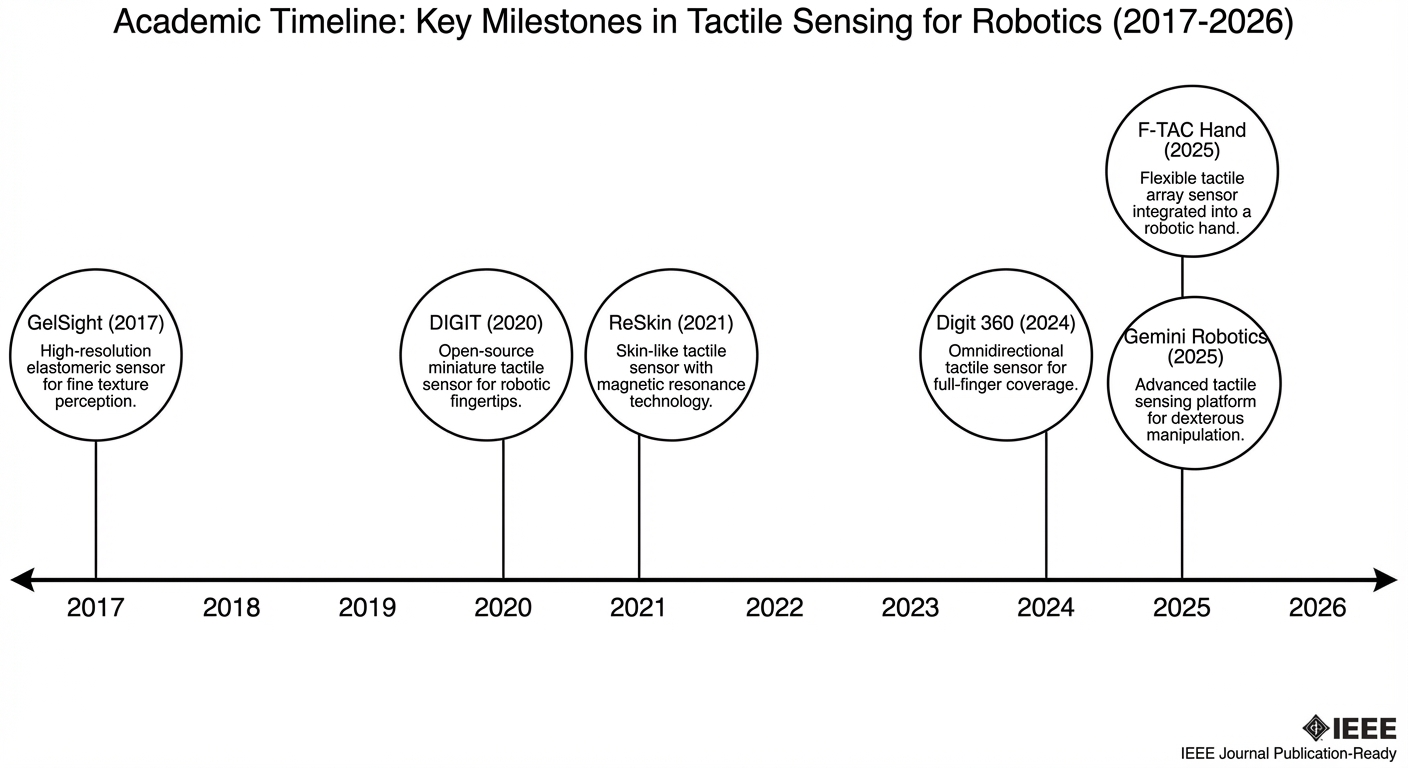
\includegraphics[width=\columnwidth]{../assets/figures/ch01/fig_1_2_timeline_academic.png}
\caption{Timeline of major milestones in tactile sensing for robot manipulation, from early transduction research through the GelSight revolution to modern VLA-based tactile integration.}
\label{fig:timeline}
\end{figure}

\subsection{Scope and Contributions}

This survey covers the full pipeline from tactile sensor hardware to learned dexterous manipulation policies, organized along six tightly coupled dimensions:
\begin{enumerate}
    \item \textbf{Tactile sensing technologies} (Section~\ref{sec:sensors}): five transduction principles, the GelSight--DIGIT--Digit~360 lineage, multi-axis sensing, and emerging neuromorphic/self-healing approaches.
    \item \textbf{Robot hand design and intelligent mechanisms} (Section~\ref{sec:hands}): the open-source ecosystem, actuation methods, and physical intelligence through underactuation, variable stiffness actuators, and active surfaces.
    \item \textbf{Data representation and collection} (Section~\ref{sec:data}): Albini et al.'s six-structure taxonomy~\cite{albini2025representing}, sensor-agnostic representations (AnyTouch~\cite{feng2025anytouch}, Canonical 3D~\cite{wu2025canonical}), public datasets, and tactile foundation models (Sparsh~\cite{higuera2024sparsh}, UniTouch~\cite{yang2024unitouch}).
    \item \textbf{Learning-based manipulation} (Section~\ref{sec:learning}): imitation learning (Diffusion Policy~\cite{chi2023diffusion}, ACT/ALOHA~\cite{zhao2023aloha}), reinforcement learning (DeXtreme~\cite{handa2023dextreme}), force-informed learning (DexForce~\cite{chen2025dexforce}, ForceVLA~\cite{yu2025forcevla}), and optimization alternatives.
    \item \textbf{VLA models} (Section~\ref{sec:vla}): from RT-1~\cite{brohan2023rt1} through pi0~\cite{black2024pi0} to Gemini Robotics~\cite{google2025gemini}, including tactile integration and post-deployment improvement via RECAP~\cite{pi2025recap}.
    \item \textbf{Human-to-robot transfer} (Section~\ref{sec:retarget}): kinematic retargeting (AnyTeleop~\cite{qin2023anyteleop}, ImMimic~\cite{liu2025immimic}), visual gap bridging (DexUMI~\cite{xu2025dexumi}), tactile gap solutions (OSMO~\cite{yin2025osmo}, UniTacHand~\cite{zhang2025unitachand}), and mechanical coupling (DEXOP~\cite{fang2025dexop}).
\end{enumerate}

We further analyze integrated systems and industrial applications (Section~\ref{sec:systems}), systematically identify the top~10 open challenges from 146 papers spanning 2020--2026 (Section~\ref{sec:discussion}), and propose the \emph{mechanism--tactile--learning triangle} as a unifying research direction for manufacturing-grade dexterous manipulation.

Our key contributions are:
\begin{itemize}
    \item The first survey to jointly cover tactile sensing hardware, dexterous hand design, VLA-based control, and embodiment retargeting within a single unified framework.
    \item A systematic identification and analysis of the top~10 open challenges based on frequency analysis across 146 recent papers.
    \item The mechanism--tactile--learning triangle: a proposed research direction that integrates physical intelligence (underactuation, VSA, active surfaces) with tactile perception and learned policies to reduce the burden on each individual axis.
\end{itemize}

\subsection{Comparison with Existing Surveys}

Several recent surveys address subsets of this space. The foundational review by Dahiya et al.~\cite{dahiya2010tactile} established the taxonomy of tactile transduction methods and remains the standard starting reference for the field. Albini et al.~\cite{albini2025representing} systematized tactile data representations into six canonical structures with selection guidelines based on hardware, task, and information requirements. Lepora~\cite{lepora2025past} traced four generations of tactile robotics history from the origins (1965--1979), through foundations and growth (1980--1994), the ``tactile winter'' (1995--2009), to the current expansion and diversification (2010--2024). The VLA systematic review~\cite{various2026vla} analyzed 102 models across 26 datasets and 12 simulation platforms, while ``What Matters in Building VLAs''~\cite{various2025whatmatters} (\emph{Nature Machine Intelligence}) found that hierarchical/late fusion architectures with diffusion decoders achieve the best generalization. A process-centric manipulation taxonomy~\cite{various2025taxonomy} (\emph{Nature Machine Intelligence}) formalized the connection from process specifications to tactile manipulation skills, validating 28 skills at near-100\% success rates.

However, \emph{no existing survey jointly covers tactile hardware, hand design, VLA-based control, and embodiment retargeting}. Sensor-focused surveys omit how sensing integrates with modern policy architectures; VLA surveys do not address the hardware and data collection dimensions; hand design reviews ignore the learning and transfer pipeline. This paper fills that gap by providing a unified treatment spanning the complete hardware--data--learning--transfer pipeline.

\subsection{Paper Organization}

The remainder of this paper is organized as follows. Section~\ref{sec:sensors} reviews tactile sensing technologies across five transduction principles. Section~\ref{sec:hands} covers robot hand design and intelligent mechanisms. Section~\ref{sec:data} addresses data representation, collection pipelines, and foundation models. Section~\ref{sec:learning} surveys learning-based manipulation including IL, RL, and force-informed approaches. Section~\ref{sec:vla} examines VLA models and their tactile integration. Section~\ref{sec:retarget} discusses embodiment retargeting. Section~\ref{sec:systems} presents integrated systems and industrial deployment. Section~\ref{sec:discussion} identifies open challenges and proposes the mechanism--tactile--learning triangle. Section~\ref{sec:conclusion} concludes.
